% Aspectratio 16:9 should be used
% The theme is not suited for 4:3 aspectratio
\documentclass[aspectratio=169]{beamer}

% Metadata of the presentation
\title{Sound separation }
\subtitle{using ad-hoc distributed microphone arrays}
\date[ISBT 2022]{}
\author[MM]{Martijn Meeldijk --- \texttt{martijn.meeldijk@ugent.be}}

% Load the UGent theme
\usetheme[language=en,faculty=ea,usecolors]{ugent}

% Have this if you'd like section slides 
\AtBeginSection[]{
    \sectionframe
}
\usepackage{graphicx}
\usepackage{mathrsfs}

\graphicspath{ {./images/} }
\usepackage{caption}
\usepackage{subcaption}
\begin{document}

% Have this if you'd like the presentation to start 
% with a large UGent logo
\logoframe

% I guess you always want a titleframe
\titleframe

% Have this if you'd like a frame containing the 
% table of content
\begin{frame}{Overview}
    \tableofcontents[hideallsubsections]
\end{frame}

% Start of the first section
\section{Introduction: Ad-hoc microphone arrays}

\begin{frame}
    \frametitle{Ad-hoc microphone arrays}
    Also known as acoustic sensor networks (ASN):
    \begin{itemize}
        \item Several microphones
        \item Unknown locations in a room
    \end{itemize}
    \vspace{.25cm}
    Increasing interest due to:
    \begin{itemize}
        \item Declining cost of receivers
        \item Edge devices such as laptops, phones, tablets
           
    \end{itemize}
\end{frame}

\begin{frame}
    \frametitle{Challenges}
    Often different nodes are only weakly synchronized
    \begin{itemize}
        \item Algorithm should be able to deal with this
    \end{itemize}
    \vspace{.25cm}
    Limited bandwidth
    \begin{itemize}
        \item Try to exchange little information
        \item Limit amount of computations
           
    \end{itemize}
\end{frame}

\begin{frame}
    \frametitle{Problems}
    Clustering
    \begin{itemize}
        \item Divide receivers into clusters dominated by a source
        \item Optional extra cluster for background noise or interference
    \end{itemize}
    \vspace{.25cm}
    Classification
    \begin{itemize}
        \item E.g. speech, music, noise, ...
    \end{itemize}
     \vspace{.25cm}
    Separation
    \begin{itemize}
        \item Enhancing the signal for a given source
    \end{itemize}
    
\end{frame}

\section{Clustering source dominated microphones}


\begin{frame}
    \frametitle{Fuzzy Clustering}
    Instead of hard clustering
     \begin{itemize}
        \item Assign fuzzy membership values (FMV)
        \item Indicates how much a microphone belongs to a cluster
           
    \end{itemize}

\end{frame}

\begin{frame}
    \frametitle{Fuzzy Clustering}
    \framesubtitle{Steps}
    Extract Mod-MFCC features
     \begin{itemize}
        \item Feature vector based on modulations om Mel-Frequency cepstral
        coeficcients
        \begin{itemize}
            \item Processed in blocks of 4s
           
        \end{itemize}
        \item Averaged over time, so behaves more stationary compared to short-time audio features.
           
    \end{itemize}

\end{frame}
\begin{frame}
    \frametitle{Fuzzy Clustering}
    \framesubtitle{Steps}
    Assign fuzzy-membership values using the Fuzzy C-means Algorithm by evaluating least-squared error functional
    \begin{equation*}
        J_m = \sum_{d=1}^D \sum_{n=1}^N (\mu_{nd})^{\alpha} \vert \vert \bold v_d - \bold u_n \vert \vert ^2_{\beta}
    \end{equation*}
      \begin{itemize}
        \item $N$ clusters
        \begin{itemize}
            \item $N$ cluster centers $ \bold u_n =( \bold u_{n,1}, \bold u_{n,2},...,\bold u_{n,A})^T $
        \end{itemize}
        \item $D$ observations $ \{\bold v_1, \bold v_2,..., \bold v_D\} $
        
        \item Weighting exponent $\alpha$ and distance norm $\vert \vert \vert \vert _{\beta}$ with weighting matrix $\beta$
        
    \end{itemize}
  

\end{frame}

\begin{frame}
    \frametitle{Fuzzy Clustering}
    \framesubtitle{Steps}
    Detecting the background cluster
    
     \begin{itemize}
    \item An extra cluster is added for microphones where background noise is dominant
    \item Microphones assigned to a source cluster should have the background  cluster as second highest FMV
        
    \end{itemize}
        
        
  

\end{frame}


\begin{frame}
    \frametitle{Fuzzy Clustering}
    \framesubtitle{Background cluster FMV}
    \begin{figure}
        \centering
        \begin{minipage}{.5\textwidth}
          \centering
          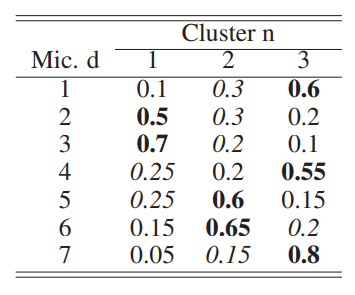
\includegraphics[width=.5\linewidth]{images/fmv1.png}
          \captionof{figure}{FMV's for each microphone}
          \label{fig:test1}
        \end{minipage}%
        \begin{minipage}{.5\textwidth}
          \centering
          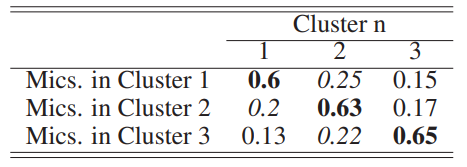
\includegraphics[width=.5\linewidth]{images/fmv2.png}
          \captionof{figure}{Average FMV's per cluster}
          \label{fig:test2}
        \end{minipage}
        \end{figure}
\end{frame}

\begin{frame}
    \frametitle{Performance}
    \framesubtitle{}
    \begin{figure}
          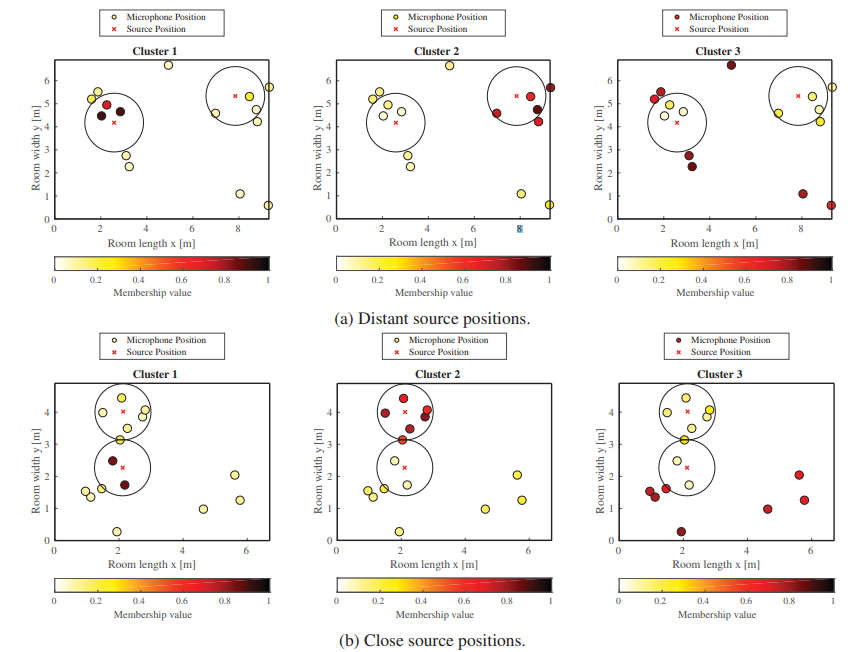
\includegraphics[width=0.7\textwidth]{images/background_clusters.png}
        \end{figure}
\end{frame}


\begin{frame}
    \frametitle{Fuzzy Clustering}
    \framesubtitle{Source separation}
      \begin{enumerate}
        \itemsep.5cm
        \item Estimate relative time-differences-of-arrival (TDOA)
        \item Combine with FMV in beamforming stage
        \item Apply cluster-related spectral masks to the output of the beamformers
        
    \end{enumerate}
   
\end{frame}

\begin{frame}
    \frametitle{Estimate relative time-differences-of-arrival}
    \framesubtitle{(TDOA)}
      \begin{itemize}

        \item Select reference microphone (highest FMV)
      \item Initial source signal estimation
              \begin{itemize}
              \item  Calculate spectral mask for reference microphone
              \item
              \begin{equation}
                  \mathscr{M}_n(k,b) = 
                  \begin{cases} 
                    1 \quad \vert X_{R_n}(k-b)\vert > \frac 1 B \sum \vert X_{R_j}(k,b)\vert, \\\ 
                    \quad \quad j = 1, \dots ,N \text{ and } j \neq n \\
                    0 \quad \text{otherwise}
                \end{cases}
              \end{equation}
              
            \item Apply to all microphones in cluster
            \end{itemize}
        
        \item Correlation analysis with respect to the reference microphone to compute TDOAs
      
        
    \end{itemize}
   
\end{frame}

\begin{frame}
    \frametitle{Clustering-steered beamforming}
    \framesubtitle{}
     \begin{equation*}
        \hat{s}_{n \text{, W-DSB}}(l) = \sum_{i_n}w_{n,i_n}x_{i_n}(l + D_{i_n})
    \end{equation*}
      \begin{itemize}

        \item  $l$: discrete time index
        \item   $D_{i_n}$: relative TDOA's
        \item $w_{n,i_n}$: the weights allocated to each microphone $i_n$ of cluster $n$
        \item These are proportional to the FMV


        \end{itemize}
        By using a weighted combination of the microphone signals, we can make a better DSB with a better output SNR than uniform weighting.
    
\end{frame}

\begin{frame}
    \frametitle{Apply cluster-related spectral masks }
    \framesubtitle{to the output of the beamformers}
      \begin{itemize}
      \item Compute a post-filtering mask, similar to what we did before
      \item
            \begin{equation}
                \mathscr{M}_n(k,b) = \begin{cases} 
            1 \quad \vert \hat S_{n, \text{FMVA-DSB}}(k,b)\vert
            > \frac 1 B \sum \vert \hat S_{j, \text{FMVA-DSB}}(k,b)\vert, \\\ 
            \quad \quad j = 1, \dots ,N \text{ and } j \neq n
            
            \\
            0 \quad \text{otherwise}
            
            \end{cases}
            \end{equation}
      \item Yields final enhanced estimate of the source signal
      
        
    \end{itemize}
   
\end{frame}

\begin{frame}
    \frametitle{Overview }
    \framesubtitle{(for two sources)}
   \begin{figure}
  
          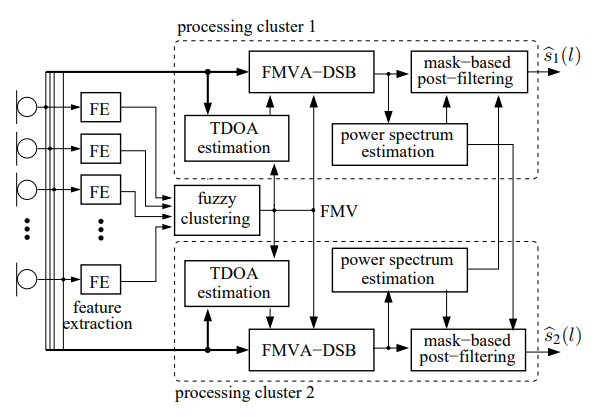
\includegraphics[width=0.5\textwidth]{images/schematic.png}
        \end{figure}
   This approach yields a slightly better performance than simple DSB.
\end{frame}
\section{Federated Learning}

\begin{frame}
    \frametitle{Federated Learning}
    Is a machine learning technique that that trains a model distributed over multiple decentralized devices. Data is not shared between nodes. Instead, a three step process is followed:

    \begin{enumerate}
        \item The clients synchronize with the server by downloading the latest model parameters
        \begin{itemize}
            \item This is a column vector $\theta^\tau$
        \end{itemize}
        \item Each client independently improves its own parameters $\theta^\tau_i$ with stochastic gradient descent on their own data
        \item Each client uploads its model parameter updates $\Delta\theta^\tau_i$ to the server, where they are aggregated.
        
        \begin{equation}
               \pmb \theta^{\tau+1} = \sum_{i=1}^M \frac{\lvert \pmb D_i \rvert}{\lvert \pmb D \rvert} \pmb \Delta \pmb \theta^\tau_i
            \end{equation}
        \begin{itemize}
            \item  $M$: number of clients
            \item $\lvert \pmb D_i \rvert$ the cardinality of the dataset of the $i$-th client
            \item $\lvert \pmb D \rvert$: the cardinality of the total dataset
        \end{itemize}
  
    \end{enumerate}
  
\end{frame}

\begin{frame}
    \frametitle{Clustered federated learning}
    \begin{block}{Problem}
        \begin{itemize}
            \item Doesn't work if the different clients' data comes from different (incongruent) distributions.
            \item There's no single set of parameter updates that can optimally minimize the loss of all clients at the same time. 
        \end{itemize}
    \end{block}
    \vspace{.5cm}
    \pause
    \begin{alertblock}{Solution}
        Cluster clients with a similar distribution and train a seperate server model for each cluster.
    \end{alertblock}
\end{frame}

\begin{frame}
    \frametitle{Clustered federated learning}
\begin{itemize}
    \item Calculate cosine similarity between update vectors of clients $i$ and $j$, represented in matrix $A$, where:
    \begin{equation}
        a_{i,j} = \frac{ \langle \pmb \Delta \pmb \theta _i, \pmb \Delta \pmb \theta _j \rangle}{ \vert\vert \pmb \Delta  \pmb \theta _i, \pmb \Delta \pmb  \theta _j \vert\vert}
    \end{equation}
    \begin{itemize}
        \item  $\langle \cdot \rangle$ denotes the inner product
        \item $\lvert \lvert \cdot \rvert \rvert$ denotes the $L_2$ norm
    \end{itemize}   
    \item Cluster hierachically using bi-partitioning
    \begin{itemize}
        \item Resulting two clusters $c_1$ and $c_2$ derived such that
        \begin{equation}
            \max_{\forall i \in c_1, k\in c_2}(a_{i,k}) < 
            \min(\min_{\forall i,j \in c_1}(a_{i,j}), \min_{\forall k,l \in c_2}(a_{i,j}))
        \end{equation}  
        \item maximum cross-cluster
cosine similarity is always smaller than the minimum of either intra-cluster cosine similarities
    \end{itemize}
\end{itemize}
\end{frame}

\begin{frame}
    \frametitle{Clustered federated learning}
\begin{itemize}
   

    \item Verification using the mean and maximum Euclidian norms of weight update vectors
    \begin{equation}
        \Delta \overline \theta_c = \Big \lVert \frac 1 {\lvert c \rvert} \sum_{i\in c} \pmb \Delta \pmb \theta_i \Big \rVert
        \text{ and }
        \Delta \hat \theta_c = \max_{i \in c}(\lVert \Delta \pmb \theta_i \rVert)
    \end{equation}
    \begin{itemize}
        \item If server reaches stationary solution but clients are still converging
        \item $\Delta \overline \theta_c$ will be low and $\Delta \hat \theta_c$ high, this prompts bi-partitioning 
    \end{itemize}
\end{itemize}
\end{frame}

\begin{frame}

\frametitle{Membership values}
    To assess contribution of each node to its respective cluster. For two clusters:
    \begin{itemize}
        \item Calculate average intra-cluster similarities for each client $i$ , arranged in vector $\pmb q$ 
        \begin{equation}
            q_i = \frac 1 {\lvert c_x \rvert - 1}\sum_{j \in c_x/i}a_{i,j}
        \end{equation}
        \item Calculate average cross-cluster similarities for each client $i$, arranged in vector $\pmb r$ 
        \begin{equation}
            r_i = \frac 1 {\lvert c_y \rvert}\sum_{k \in c_y}a_{i,k}
        \end{equation}
        \item $\forall i \in c_x$  and $(c_x, c_y) \in \{ (c_1, c_2), (c_1, c_1) \}$, where $\lvert \cdot \rvert$ denotes the cardinality
    \end{itemize}
    
\end{frame}

\begin{frame}
\frametitle{Membership values}
    
    \begin{itemize}
    \item Now apply min-max normalization to obtain vector $\pmb p$ with:
    \begin{equation}
        p_i = \lambda \frac{q_i - \min(\pmb q) }{\max(\pmb q) - \min(\pmb q)}
+ (1- \lambda) \frac{r_i - \min(\pmb r) }{\max(\pmb r) - \min(\pmb r)}
    \end{equation}
    \item Select the node with the smallest $p_i$ as reference node
    \item The membership value of a node is the cosine similarity between this node and the reference node
    \begin{equation}
        \mu_i = a_{i, \arg \min(p_j)}, \forall i,j \text{ and } c_x \in \{c_1, c_2\}
    \end{equation}
     \item Now, apply min-max normalization again to the vector $\pmb \mu$
    
    \end{itemize}
    
\end{frame}

\begin{frame}
\frametitle{Cluster membership values}
\begin{figure}
    \centering
    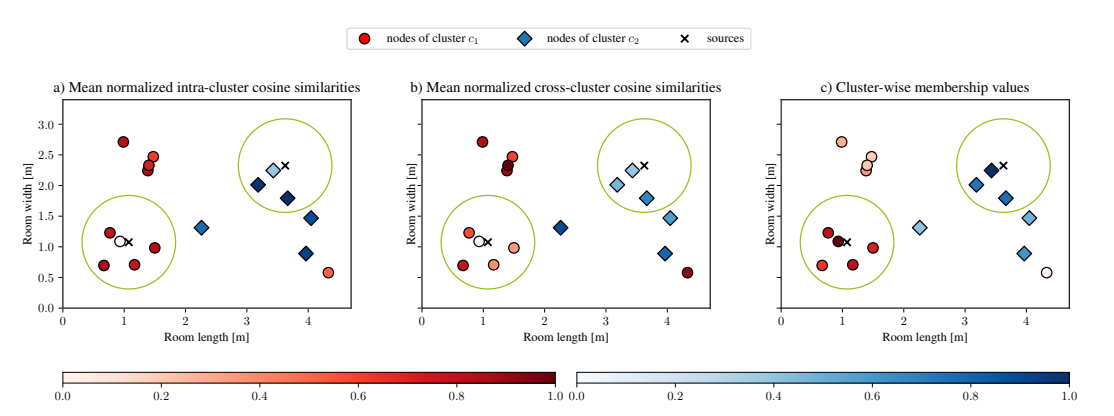
\includegraphics[width=.9\linewidth]{images/federated.png}
    \caption{FMV's for unsupervized CFL}
    \label{fig:federated}
\end{figure}
    
\end{frame}

\section{Coherence-based clustering}

\begin{frame}
\frametitle{Coherence-based clustering}
\framesubtitle{With non-negative matrix factorization}
\begin{itemize}
    \item A signal consisting of clean speech and interference:
    \begin{equation}
        x_m(t) = s_m(t) + v_m(t)
    \end{equation}
    \item We'll consider the signal as a frame of observation samples in vector form
    \begin{align*}
        \pmb x_m(t) &= [x_m(t)x_m(t - 1) \cdots x_m(t - T + 1)]T  \\
        &= \pmb s_m(t) + \pmb v_m(t)
    \end{align*}
    \item With $T$ denoting frame size
    
\end{itemize}
\end{frame}

\begin{frame}
\frametitle{Coherence-based clustering}
\framesubtitle{With non-negative matrix factorization}

The proposed clustering algorithm works in two steps:
\begin{enumerate}
    \item Compute the magnitude squared coherence between the microphone observations to measure their degree of linear dependency
    \item Apply NMF to the output of the previous step to find the optimal clustering
\end{enumerate}
\end{frame}


\begin{frame}
\frametitle{Magnitude-squared coherence}

\begin{itemize}
    \item We can measure the coherence between two signals $x(t)$ and $y(t)$ by computing the FFT of the signals. 
    \item Then, we measure the coherence as a function of the center frequency of the filter.
    \begin{equation}
        \Gamma_{xy}(f) = \frac{\lvert S_{xy}(f)\rvert ^2}{S_{xx}(f)S_{yy}(f)}
    \end{equation}
    \item $S_{xy}(f)$ is the cross-spectral density, which is really a spectral correlation density. This tells how the two signals are correlated in the time domain at a certain frequency and can be computed as:
    \begin{equation}
        S_{xy}(f) = \sum_{k=1-T}^{T-1} R_{xy}(k)e^{-i2\pi fk}
    \end{equation}
\end{itemize}
\end{frame}

\begin{frame}
\frametitle{Magnitude-squared coherence}
$R_{xy}(k)$ from the previous slide is the cross-correlation function between $x(t)$ and $y(t)$ and can be estimated by:
\begin{equation}
    R_{xy}(k) = 
    \begin{cases}
    \frac 1T \sum_0^{T-1-k} x(t)y(t+k)  &k=0,\dots,T-1 \\
    R_{xy}(-k)  &k=-(T-1),\dots,-1 \\

\end{cases}
\end{equation}
    
\end{frame}

\begin{frame}
\frametitle{Magnitude-squared coherence}

Now we'll make a matrix consisting of all the correlations between the different microphone signals. We'd like to give the same weight to all frequency bins, regardless of their power. So we'll use the following coherence metric:

    \begin{equation}
    C_{xy} = \frac{\sum_{f=0}^{F} \Gamma_{xy}(f)}{F} \in [0,1]
    \end{equation}
    \begin{itemize}
        \item With $F$ denoting the number of frequency bins
    \end{itemize}
    Arranging all of the coherence measures between observations into a matrix, we obtain $\pmb C$
    \begin{equation}
        \pmb C=
        \begin{bmatrix}
        1 & \cdots & \cdots & C_{1M} \\
        C_{12} & 1 & \cdots &\vdots \\
        \vdots& \vdots& \ddots &\vdots \\
        C_{1M} & C_{2M} & \cdots & 1
        \end{bmatrix}
    \end{equation}
    
\end{frame}

\begin{frame}

\frametitle{Non-negative matrix factorization}

    \begin{itemize}
        \item Every value $C_{ij}$ contains the degree of correlation between the $i$-th and $j$-th observation. This means that microphones close to a certain source will be correlated.
        \item  The matrix $\pmb C$ can be modelled as:
        \begin{equation}
            \pmb C = \pmb B \pmb B^T \odot (\pmb 1- \pmb I) + \pmb I
        \end{equation}
        \begin{itemize}
            \item $B \in \mathbb{R}^{M \times K}$ is the cluster matrix, where $K$ is the amount of speakers (the amount of clusters)
            \item Because $\pmb C$ is symmetric, we model it as $\pmb B \pmb B^ T$
            \item $\odot$ is the element-wise product
            \item $\pmb I$ is the identity matrix 
            \item $ \pmb 1$ is the all-ones matrix
            \item The latter two are introduced because the main diagonal of $\pmb C$ does not provide any relevant information in the learning process of $\pmb B$
        \end{itemize}
    \end{itemize}
\end{frame}

\begin{frame}
\frametitle{Non-negative matrix factorization}

    \begin{itemize}
        \item Based on Euclidian divergence, $\pmb B$ is estimated with multiplicative update rules. It is first initialized with random values in the algorithm:
        \begin{equation}
            \pmb B \leftarrow \pmb B \odot \frac{(\pmb C \odot (\pmb 1- \pmb I)) \pmb B}{(\pmb B \pmb B^{\pmb T} \odot (\pmb 1 - \pmb I)) \pmb B}
        \end{equation}
        \item Now each column of $\pmb B$ contains the contribution of a microphone to each cluster. We can obtain the clustering result with:
        \begin{equation}
            \gamma_m = 
            \{ j \in [1,K] : B_{mj} \geq B_{mk}, \forall k \in [1,K] \}
        \end{equation}
        \item $\gamma_m $ denotes the cluster assigned to the $m$-th microphone. This is simply the largest value of column $m$.
    \end{itemize}
    For those wondering, the variance ratio criterion (VRC) is used to obtain the optimal number of clusters
\end{frame}



\begin{frame}
\frametitle{Non-negative matrix factorization}
\framesubtitle{Results}


\begin{figure}
    \centering
    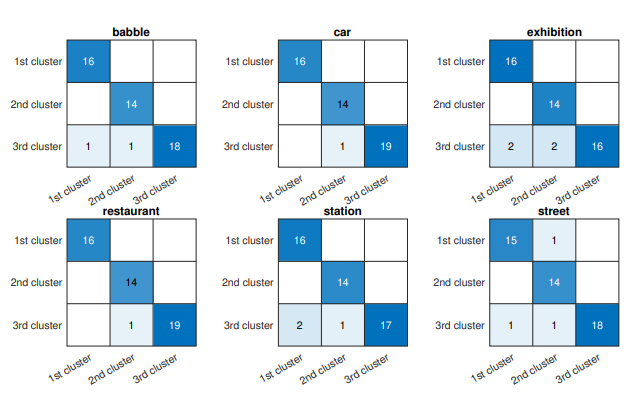
\includegraphics[width=.6\linewidth]{images/200ms.png}
    \caption{Confusion matrix for a simulation with 3 clusters and 50 microphones. For reverberation time $T_{60} = 200 \space ms$}
    \label{fig:my_label}
\end{figure}
    
\end{frame}


\begin{frame}
\frametitle{Non-negative matrix factorization}
\framesubtitle{Results}


\begin{figure}
    \centering
    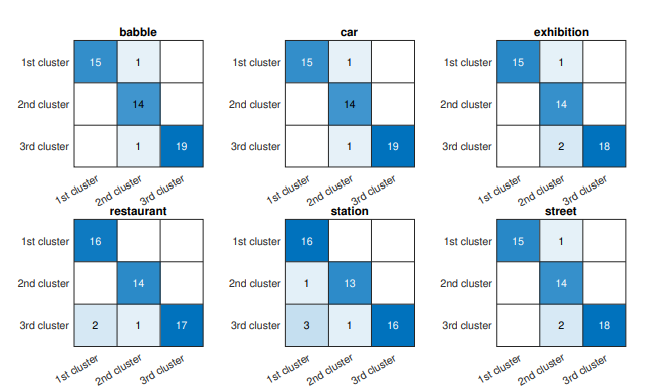
\includegraphics[width=.6\linewidth]{images/400ms.png}
    \caption{Confusion matrix for a simulation with 3 clusters and 50 microphones. For reverberation time $T_{60} = 400 \space ms$}
    \label{fig:my_label}
\end{figure}

    
\end{frame}



\begin{frame}
\frametitle{Non-negative matrix factorization}
\framesubtitle{Conclusion}

    \begin{itemize}
        \item Allows clustering without any prior knowledge of the acoustic scene
        \item Improved clustering performance in comparison to other methods
    \end{itemize}

\end{frame}

\begin{frame}{Overview}
    \tableofcontents[hideallsubsections]
\end{frame}


\section{Questions?}

% End presentation with titleframe
\titleframe

\end{document}
